\chapter{Clase 2}
\clasedate{02 de abril de 2025}
\section{Equivalante Norms}
Teníamos que, $\forall\, x \in \Rn$,
$$
	\norm{x}_{\infty} \leq \norm{x}_2 \leq \norm{x}_1 \leq n \norm{x}_{\infty}
$$
Estas tres normas son equivalentes.

Dada $(x_k)_{k \in \N} \subset \Rn$, con $\forall \, k\in \N, x_k = (k_1^k, \, x_2^k, \ldots, x_n^k) \in \Rn, \; a = (a_1, \ldots ,a_n)\in \Rn$

$
	\lim\limits_{k \to \infty} x_k = a $ significa que $\forall\; \varepsilon>0,\, \exists k_0 \in \N, \, \forall k \in \N
$
\begin{align*}
	k \geq k_0 \longrightarrow & \norm{x_k-a} < \varepsilon                                      \\
	                           & \abs{ \norm{x_k-a}-0} < \varepsilon,  \quad \norm{x_k-a} \in \R
\end{align*}

\thmr{Equivalencia de la convergencia en \(\mathbb{R}^n\)}{teorema3}{
	Sea \( (x_k)_{k \in \N} \subset \mathbb{R}^n \) y \( a \in \mathbb{R}^n \). Entonces:
	$$
		\lim_{k \to \infty} x_k = a \quad \text{en } \norm{\cdot}_2
		\iff
		\forall i \in \{1, \ldots, n\}, \quad \lim_{k \to \infty} x_i^k = a_i
	$$
}

\pf{Prueba del teorema \ref{thm:teorema3}\\
	Sea una subsucesión $(x_k)_{k\in \, \N}=(x_1, x_2, x_3, x_4, x_5, x_6, x_7, \ldots) \subset \Rn $,

	\begin{itemize}
		\item Una subsucesión de \((x_k)_{k \in \mathbb{N}}\) es una sucesión de la forma:
		      \[
			      (x_{i_k})_{k \in \mathbb{N}} = (x_{i_1}, x_{i_2}, x_{i_3}, \ldots)
		      \]
		      tal que $(i_k)_{k \in \mathbb{N}} \subset \mathbb{N}, \{i_1< i_2< i_3< \ldots\} = \N' \subset \N$, es estrictamente creciente.

		      \begin{itemize}
			      \item Función de índices:
			            \begin{align*}
				            i \colon \N & \longrightarrow \N   \\
				            k           & \longmapsto i(k)=i_k
			            \end{align*}

			      \item Sucesión original como función:
			            \begin{align*}
				            x \colon \N & \longrightarrow \Rn  \\
				            k           & \longmapsto x(k)=x_k
			            \end{align*}
			      \item Subsucesión como composición:
			            \begin{align*}
				            x \circ i \colon \N & \longrightarrow \Rn                            \\
				            k                   & \longmapsto (x \circ i)(k) = x(i(k)) = x_{i_k}
			            \end{align*}
			      \item Notación alternativa para la subsucesión:
			            \[
				            (x_{i_k})_{k \in \N} = (x_p)_{p \in \N'}, \quad \text{donde } \N' = \{i_1, i_2, i_3, \ldots\} \subset \mathbb{N}
			            \]
		      \end{itemize}
		\item   Sea \(X \subset \mathbb{R}^n\). Decimos que \(X\) es \textbf{acotado con respecto a la norma infinito}

		      \begin{equation}
			      \exists \; c>0 \text{ tal que } X \subset B^{\norm{\cdot}_\infty}(\vb{0}, c) = \left\lbrace z \in \mathbb{R}^n : \norm{z - \vb{0}}_\infty \leq c \right\rbrace
			      \label{eq:norm-infty-ball}
		      \end{equation}
		      \[
			      B^{\norm{\cdot}_\infty}(\vb{0}, c) = \left\lbrace z = (z_1, \ldots, z_n) \in \mathbb{R}^n : \max_{1 \leq i \leq n} |z_i| \leq c \right\rbrace
		      \]
		      \[
			      B^{\norm{\cdot}_\infty}(\vb{0}, c) = [-c, c]^n = \prod_{i=1}^n [-c, c].
		      \]

		      Por lo tanto, la condición de acotamiento se puede expresar también como:

		      \[
			      \exists\, c > 0 \text{ tal que } \forall\, x \in X,\quad \norm{x}_\infty \leq c.
		      \]

		      %Es decir, todos los vectores \(x = (x_1, \ldots, x_n) \in X\) tienen cada componente dentro del intervalo \([-c, c]\), o equivalentemente:
		      \[
			      |x_i| \leq c,\quad \text{para todo } i = 1, \ldots, n.
		      \]
		      \begin{figure}[H]
			      \centering
			      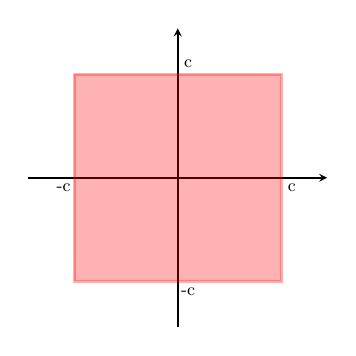
\begin{tikzpicture}[scale=0.7]
				      \begin{axis}[
						      width=7cm, height=7cm,
						      axis lines=middle,
						      xtick=\empty, ytick=\empty,
						      axis equal,
						      enlargelimits,
						      xmin=-1.2, xmax=1.2,
						      ymin=-1.2, ymax=1.2,
						      thick,
						      domain=0:90
					      ]

					      %p=inf
					      \draw[ultra thick, red!100!blue, fill=red!100!blue, opacity=0.3 ] (axis cs:-1,-1) rectangle (axis cs:1,1);

					      % Add +1 and -1 labels
					      \node[font=\small] at (axis cs:1.1,-0.1) {c};
					      \node[font=\small] at (axis cs:-1.1,-0.1) {-c};
					      \node[font=\small] at (axis cs:0.1,1.1) {c};
					      \node[font=\small] at (axis cs:0.1,-1.1) {-c};

				      \end{axis}
			      \end{tikzpicture}
		      \end{figure}
	\end{itemize}
}


\prop{
	Sea \(X \subset \mathbb{R}^n\). Entonces:

	\[
		X \text{ es acotado (en } \norm{\cdot}_\infty) \iff \forall\, i \in \{1, \ldots, n\},\ \pi_i(X) \text{ está acotado en } \mathbb{R},
	\]
	donde \(\pi_i\colon \mathbb{R}^n \to \mathbb{R}\) es la proyección sobre la \(i\)-ésima coordenada.

}
\pf{   \((\Rightarrow)\)  Supongamos que \(X \subset \mathbb{R}^n\) es acotado en la norma infinito.

Entonces, existe \(c > 0\) tal que:
\[
	X \subset B^{\norm{\cdot}_\infty}[0, c] = \{x \in \mathbb{R}^n : \norm{x}_\infty \leq c \} = \prod_{i=1}^n [-c, c].
\]

De esto se deduce que para cada \(i \in \{1, \ldots, n\}\), la proyección \(\pi_i(X)\) satisface:
\[
	\pi_i(X) \subset [-c, c],
\]
es decir, cada coordenada de los vectores en \(X\) está acotada por \(c\).

\((\Leftarrow)\)  (Ejercicio)

}

\thmr{Bolzano–Weierstrass en $\Rn$}{teorema4}{
	Sea \( (x_k)_{k \in \mathbb{N}} \subset \mathbb{R}^n \) una sucesión acotada.
	Entonces, existe una subsucesión \( (x_{k_j})_{j \in \mathbb{N}} \) y un punto \( x \in \mathbb{R}^n \) que  convergen
	\[
		\lim_{j \to \infty} x_{k_j} = x.
	\]
}

\pf{ Prueba del Theorem \ref{thm:teorema4}\\
\underline{Caso $n=3$:}
\begin{itemize}
	\item Como $(x_k)_{k \in \N}$ es acotada $\rightarrow \exists \, c>0$ tal que $x_k = (x_1^k, \, x_2^k, \, x_3^k) \in \Real{3}$

	      $(x_1^k)_{k \in \N} \subset \R $ es acotado, pues

	      \begin{equation}
		      \forall\, k \in \N, \norm{x_k}_{\infty} \leq c\rightarrow \abs{x_i^k} \leq c, \quad \forall\, i \in \qty{1, 2, 3}
		      \label{eq:teorema4_1}
	      \end{equation}

	      Por \textbf{Bolzano-Weierstrass en $\R$}, $\exists \, (x_1^{i_k})_{k \in \N} \subset ( x_1^k)_{k \in \N}$ tal que $\lim\limits_{k \to \infty} x_1^{i_K} = b_1 \in \R $\\
	      donde $i_1<i_2< i_3<\ldots$

	\item $(x_2^{i_k}) \subset (x_2^k)_{k\in \N}$ es acotada, pues $\abs{x_2^k} \leq c, \forall\, k \in \N$

	      Por \textbf{Bolzano-Weierstrass en $\R$}, $\exists \, (x_2^{i_{j_k}})_{k \in \N} \subset ( x_2^{i_k})_{k \in \N}$ tal que $\lim\limits_{k \to \infty} x_2^{i_{j_K}} = b_2 \in \R $

	\item  $(x_3^{i_{j_k}})   $ es acotada por \eqref{eq:teorema4_1}

	      Por \textbf{Bolzano-Weierstrass en $\R$}, $\exists \, (x_3^{i_{j_{p_k}}})_{k \in \N} \subset ( x_3^{i_{j_k}})_{k \in \N}$ tal que $\lim\limits_{k \to \infty} x_3^{i_{j_{p_k}}} = b_3 \in \R $
\end{itemize}
Como $(x_1^{i_{j_{p_k}}})_{k \in \N} \subset (x_1^{i_k})_{k \in \N}$ y $(x_2^{i_{j_{p_k}}})_{k \in \N} \subset (x_2^{i_k})_{k \in \N}$ entonces
$$
	\lim\limits_{k \to \infty} x_1^{i_{j_{p_k}}}=b_1 \in \R
$$
$$
	\lim\limits_{k \to \infty} x_2^{i_{j_{p_k}}}=b_2 \in \R
$$
$$
	\lim\limits_{k \to \infty} x_3^{i_{j_{p_k}}}=b_3 \in \R
$$
Del theorem \ref{thm:teorema3}
$$
	\pqty{x_{i_{j_{p_k}}}} _{k\in \N} \text{ converge } (b_1, b_2, b_3)
$$
donde,
$$
	x_{i_{j_{p_k}}}=\pqty{x_1^{i_{j_{p_k}}}, x_2^{i_{j_{p_k}}}, x_3^{i_{j_{p_k}}}}, \forall k \in \N
$$
}

Sabemos que \( (\mathbb{R}, |\cdot|) \) es un espacio métrico completo.

\begin{itemize}
	\item Sea \( (x_k)_{k \in \mathbb{N}} \subset \mathbb{R}^n \) una sucesión.
	      Entonces, \( (x_k) \) es de Cauchy en \( \mathbb{R}^n \) (respecto a alguna norma \( \|\cdot\| \)) si y solo si:
	      \[
		      \forall\, \varepsilon > 0,\ \exists\, k_0 \in \mathbb{N}\ \text{tal que}\ \forall\, m, p \in \mathbb{N},\ m, p \geq k_0 \Rightarrow \|x_m - x_p\| < \varepsilon.
	      \]
\end{itemize}

\ex{Si $(x_{k})_{k \in \N} \subset  \Rn$ es convergente $\rightarrow (x_k)_{k\in \N}$ es de Cauchy.
	\pf{
		Sea $(x_k)_{k\in \N}$ sucesión convergente en $\Rn$
		$$
			\rightarrow \exists \, a \in \Rn \text{ tal que } \lim\limits_{k \to \infty } x_k =a
		$$
		Dado $\varepsilon >0, \exists\, k_0 \in \N$
		\begin{align*}
			k\geq k_0 & \rightarrow \norm{x_k-a} < \frac{\varepsilon}{2} \\
			p\geq k_0 & \rightarrow \norm{x_p-a} < \frac{\varepsilon}{2}
		\end{align*}
		\begin{align*}
			\text{Si }	k, p \geq k_0 \rightarrow \norm{x_k-k_p} & \leq \norm{x_k-a}+\norm{a-x_p}                 \\
			                                                    & < \frac{\varepsilon}{2}+ \frac{\varepsilon}{2} \\
			\norm{x_k-k_p}                                      & <\varepsilon
		\end{align*}
		$\therefore (x_{k})_{k \in \N} $ es de Cauchy.
	}
}


\thmr{}{teorema5}{
El espacio \( (\mathbb{R}^n, \|\cdot\|_{\infty}) \) es completo.

Es decir, si \( (x_k)_{k \in \mathbb{N}} \subset \mathbb{R}^n \) es una sucesión de Cauchy respecto a \( \|\cdot\|_{\infty} \), entonces \( (x_k) \) converge en \( \mathbb{R}^n \).
}

\pf{
	Prueba del teorema \ref{thm:teorema5} \\
	Sea $x_k = \pqty{x_1^k, x_2^k, \ldots, x_n^k}, \forall\, k\in \N$ tal que $(x_k)_{k \in \mathbb{N}}$ es de Cauchy.

	Dado $\varepsilon >0,  \exists \, k_0 \in \N \quad \forall k, p \in \N$
	\begin{align*}
		k, p \geq k_0 \longrightarrow \norm{x_k-x_p}_{\infty} & <\varepsilon \\
		\max\limits_{1 \leq i \leq n} \abs{x_i^k-x_i^p}       & \varepsilon
	\end{align*}
	$\forall i \in \{1, 2, \ldots, n\}, \quad k, p \geq k_0 \rightarrow \abs{x_{i}^{k}-x_i^p}<\varepsilon$

	$\therefore \pqty{x_i^k}_{k\in \N} \subset \R$ es de cauchy en $\R$ completo $\forall i \in \{1, \ldots, n\} \quad \exists\, a_i \in \R$ tal que $\lim\limits_{k \to \infty} x_i^k = a_i$

	del teorema \ref{thm:teorema3} \quad $\lim\limits_{k \to \infty} x_k = a = (a_1, \ldots, a_n)$

}

\thmr{Equivalencia de normas en \( \mathbb{R}^n \)}{teorema6}{
	En \( \mathbb{R}^n \), todas las normas son equivalentes.

	Es decir, dadas dos normas \( \abs{.} \) y \( \norm{.} \) en \( \mathbb{R}^n \), existen constantes \( \alpha, \beta \in \mathbb{R}^+ \) tales que:
	\[
		\forall\, x \in \mathbb{R}^n,\quad \alpha  \abs{x} \leq \norm{x}  \leq \beta \abs{x}
	\]
}

\pf{
	Prueba del teorema \ref{thm:teorema5} \\
	Basta con mostrar que cualquier norma $\abs{.}$ es equivalente a $\norm{.}_1$

	Sea $\abs{.}$ una norma en $\Rn, \forall \, x \in \Rn$,$\forall x=(x_1, \ldots, x_n)=\pqty{x_1 e_1+\cdots +x_n e_n} \in \Rn$
	\begin{align*}
		\abs{x} = \abs{\sum_{i=1}^{n} x_i e_i} \leq \sum_{i=1}^{n}\abs{x_i}\abs{e_i} & \leq \beta \sum_{i=1}^{n} \abs{x_i} \\
		                                                                             & \leq \beta \norm{x_i}_1
	\end{align*}
	donde $\max\limits_{1 \leq i \leq n} \abs{e_i}=\beta$
	\begin{equation}
		\forall \, x \in \Rn, \abs{x} \leq \beta\norm{x}_1
		\label{eq:norma_equival}
	\end{equation}

	Solo falta demostrar que $\exists \,\alpha>0, \forall\, x \in \Rn, \quad\alpha \norm{x}_1 \leq \abs{x}$

	Por contradicción, supongamos que
	$$
		\forall \,\alpha>0, \exists\, x \in \Rn, \quad\alpha \norm{x_{\alpha}}_1 > \abs{x_\alpha}
	$$
	para
	$$
		\alpha = \frac{1}{k}, \exists\, x_k \in \Rn, \frac{1}{k} \norm{x_k}_1>\abs{x_k}
	$$
	$$
		\forall k \in \N,    \exists\, x_k \in \Rn, \frac{1}{k} \norm{x_k}_1>\abs{x_k} \rightarrow x_k \neq 0
	$$
	Hemos construido $(x_k)_{k\in \N } \subset \Rn$ tal que $\norm{x_k}_1>0 \wedge \abs{x_k}>0$

	$$
		\forall k \in \N, \frac{1}{k} > \frac{1}{\norm{x_k}_1}\cdot \abs{x_k} = \abs{\frac{1}{\norm{x_k}_1}\cdot x_k} = \abs{z_k}
	$$

	Tenemos,
	\begin{align}
		\forall k \in \N, \quad\norm{z_k}_1 =1 \label{eq:equi-7} \\
		\forall k \in \N, \quad\abs{z_k}  =\frac{1}{k} \label{eq:equi-8}
	\end{align}
	Como $(z_k)_{k \in \N} \subset \Rn$, de \ref{eq:equi-7}  es acotada respecto a $\norm{.}_1$

	Por \textbf{Bolzano-Weierstrass en $\Rn$}, $\exists (z_{i_k}) \subset (z_k)_{k\in \N}$

	Para  $\norm{.}_1 \approx \norm{.}_{\infty}$ y  $\exists \, a \in \Rn$ tales que
	$$
		\lim\limits_{k\to \infty} z_{i_k}=a
	$$
	\begin{equation}
		\lim\limits_{k\to \infty} \norm{ z_{i_k} -a }=0 \label{eq:norma_equival-1}
	\end{equation}

	\rmkb{
		$$
			\norm{b} = \norm{b-c+c}\leq \norm{b-c}+\norm{c}
		$$
		$$
			\norm{b} -\norm{c}  \leq \norm{b-c}
		$$
		$$
			\rightarrow \abs{\norm{b} -\norm{c} } \leq \norm{b-c}
		$$

		$$
			\rightarrow 0 \leq \abs{\norm{z_{i_K}}_1 -\norm{a}_1 }  \leq \norm{ z_{i_k} -a }
		$$
		$$
			0 \leq \lim\limits_{k\to \infty} \abs{\norm{z_{i_K}}_1 -\norm{a}_1 }  \leq \lim\limits_{k\to \infty} \norm{ z_{i_k} -a } =0
		$$
		$$
			\rightarrow   \lim\limits_{k\to \infty} \abs{\norm{z_{i_K}}_1 -\norm{a}_1 }    =0
		$$
		$$
			\therefore   \lim\limits_{k\to \infty}  \norm{z_{i_K}}_1 =\norm{a}_1    \rightarrow a \neq 0
		$$
	}

	De \eqref{eq:norma_equival} y \eqref{eq:norma_equival-1}, como $\forall\, k \in \N, \quad \abs{z_{i_k}-a}\leq \beta\norm{z_{i_k}-a}_1 $

	$$
		\rightarrow  \lim\limits_{k\to \infty} \abs{z_{i_k}-a} = 0
	$$
	como $   \abs{\abs{z_{i_k} -\abs{a} }}\leq \abs{z_{i_k}-a}$
	$$
		\rightarrow  \lim\limits_{k\to \infty} \abs{z_{i_k}}=\abs{a}
	$$
	De \eqref{eq:equi-8}, $\abs{z_{i_k} }< \frac{1}{i_k}$
	$$
		\lim\limits_{k \to \infty} \abs{z_{i_k}} = 0 \rightarrow \abs{a}=0
	$$
	$\rightarrow a=0$ (Contradicción)

	Por lo tanto, existe \( \alpha > 0 \) tal que:

	\[
		\alpha \|x\|_1 \leq \abs{x}, \quad \forall\, x \in \mathbb{R}^n.
	\]
}

\cor{
	Sean $(x_k)_{k\in \N}$ y $(y_k)_{k\in \N}$ sucesiones en $\R^n$ tales que
	$$
		\lim_{k \to \infty} x_k = a \in \R^n \quad \text{y} \quad \lim_{k \to \infty} y_k = b \in \R^n.
	$$
	Sea $(\lambda_k)_{k\in \N} \subset \R$ una sucesión tal que $\lim_{k \to \infty} \lambda_k = \lambda_0$.

	Entonces, se cumple:
	\begin{description}
		\item[(i)]
		      \[
			      \lim_{k \to \infty} (x_k + y_k) = \lim_{k \to \infty} x_k + \lim_{k \to \infty} y_k = a + b.
		      \]

		\item[(ii)]
		      \[
			      \lim_{k \to \infty} (\lambda_k x_k) = \lambda_0 \cdot \lim_{k \to \infty} x_k = \lambda_0 a.
		      \]

		\item[(iii) Producto interno euclidiano]
		      \[
			      \lim_{k \to \infty} \inner{x_k}{y_k} = \inner{\lim_{k \to \infty} x_k}{\lim_{k \to \infty} y_k} = \inner{a}{b}.
		      \]

		\item[(iv) Para toda norma $\|\cdot\|$ en $\R^n$]
		      \[
			      \lim_{k \to \infty} \|x_k\| = \|\lim_{k \to \infty} x_k\| = \|a\|.
		      \]
	\end{description}
	Donde $a = (a_1, \ldots, a_n)$, $b = (b_1, \ldots, b_n)$, $x_k = (x_1^k, \ldots, x_n^k)$ y $y_k = (y_1^k, \ldots, y_n^k)$.
}



\pf{Prueba del ítem (i):\\
	Como $\lim\limits_{k \to \infty} x_k = a$, se tiene que, para cada $i \in \{1, \ldots, n\}$, $
		\lim\limits_{k \to \infty} x_i^k = a_i $

	Analogamente, $\lim\limits_{k \to \infty} y_i^k = b_i \quad \text{para todo } i \in \{1, \ldots, n\}$

	Por tanto, para cada $i \in \{1, \ldots, n\}$:
	\[
		\lim_{k \to \infty} (x_i^k + y_i^k) = \lim_{k \to \infty} x_i^k + \lim_{k \to \infty} y_i^k = a_i + b_i.
	\]
	Por el teorema \eqref{thm:teorema3},
	\[
		\lim_{k \to \infty} (x_k + y_k) = a + b.
	\]
}



